\chapter{実装}
%ラズパイマウスのfollowerノードについての実装を書く.今はspheroとラズパイマウスのwiibordを本実装として話しているため改変が必要.aproachに持っていく.
\begin{figure}[ht]
    \centering
    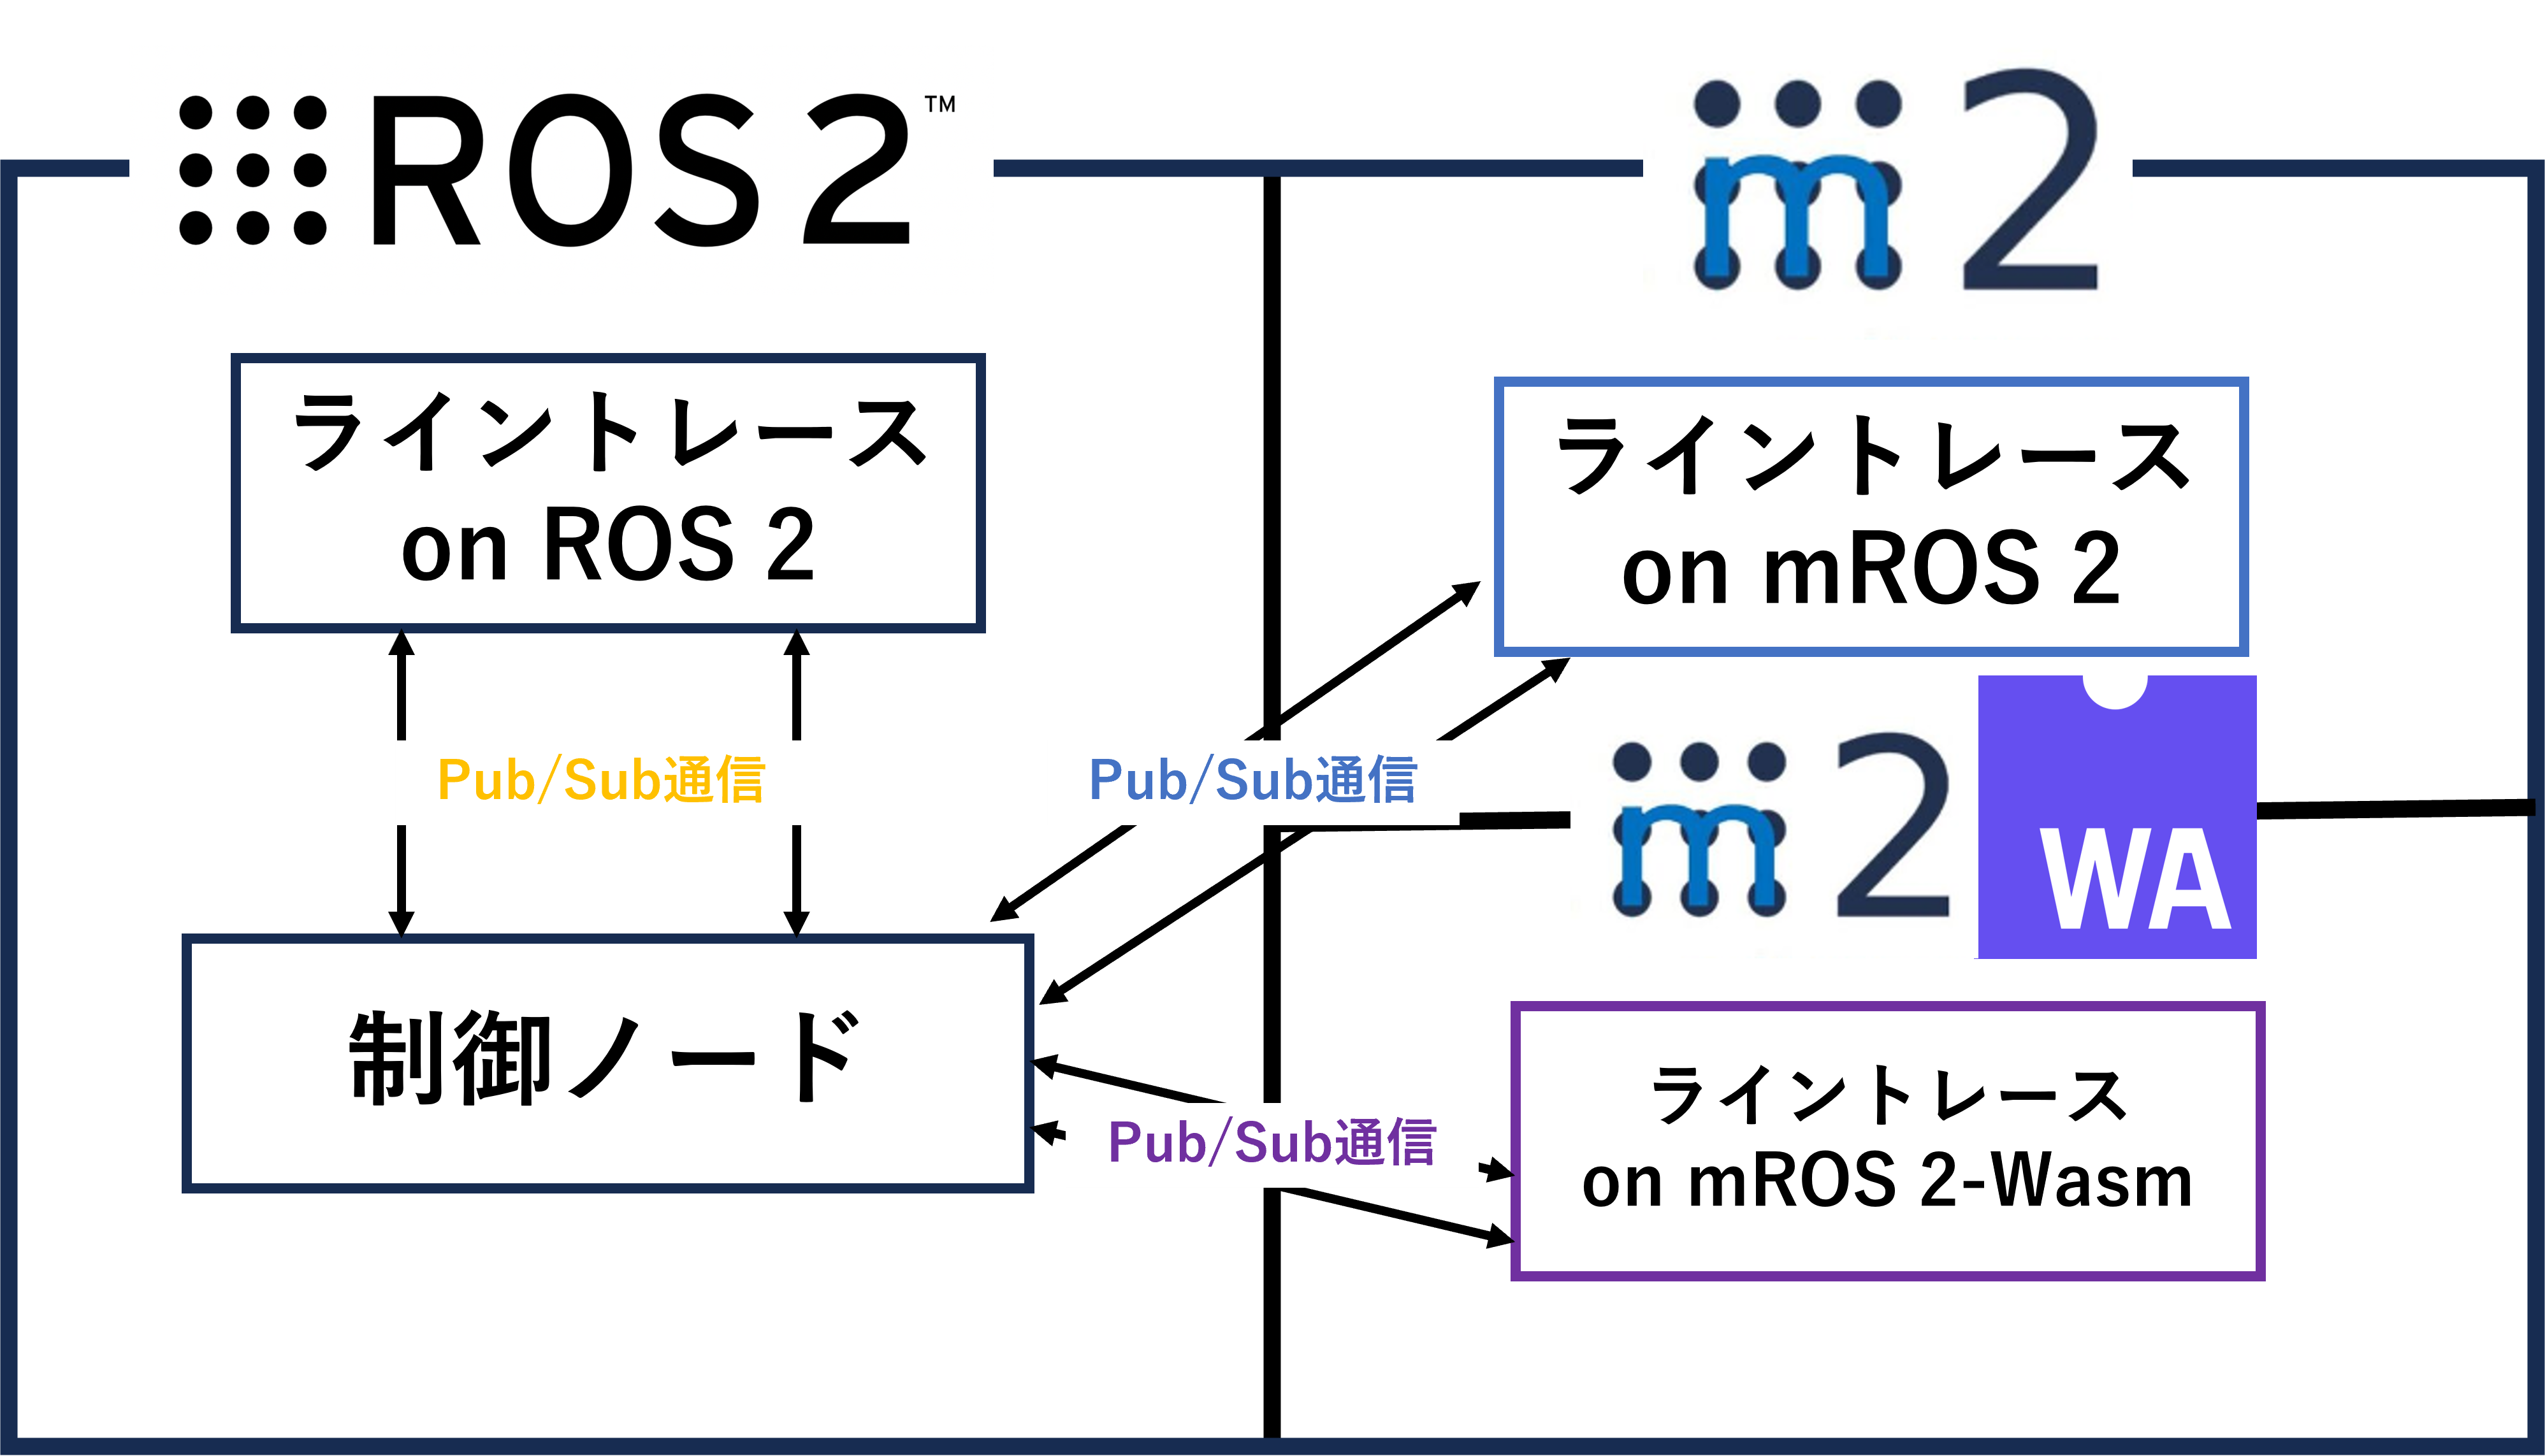
\includegraphics[width=10cm]{images/fig4_mros2_ros2_raspimouse_configuration.png}
    \caption{Raspberry Pi Mouseを制御するアプリケーションの構成図}
    \label{fig:raspimouse_configuration}
\end{figure}
\label{chap:implementation}
本章では,mROS 2-POSIXとROS 2の性能を比較評価するにあたって,mROS 2-POSIXとROS 2に実装するアプリケーションの概要について説明する.
\section{実装アプリケーションの概要}
本研究ではROS 2で動作するライントレースノードをmROS 2-POSIXに移植し,mROS 2-POSIXとROS 2の性能を比較評価する.
比較評価のためのアプリケーションの構成図を図4.1に示す.
ライントレースノードは,Raspberry Pi Mouseのセンサから取得した値をもとに,ラズパイマウスをライントレースさせるノードである.
動作フローを図4.2に示す.
まず,Switchを介してライトセンサの値を取得する動作を行う.
プログラム上で保持するライトセンサの値はラインの外側の値と,ラインの内側の値の2つである.
その後,保持した2つの差を基準にしてラインの外側にいるか内側にいるかを判断し,ラインの外側にいる場合はラインの内側に向かって旋回する動作を行う.
この動作を行うノードをmROS 2-POSIXとROS 2で実装し,比較評価を行う.
\section{実装アプリケーションの詳細}
本節では,実装アプリケーションの詳細について説明する.
ROS 2,mROS 2-POSIXで実装するノードはサブスクライブするトピックが2つ,パブリッシュするトピックが3つある.
サブスクライブするトピックは/light\_sensorsと/switchsである.
このトピックはラズパイマウス制御ノードが現在のライトセンサの値とスイッチの値をパブリッシュするトピックである.
light\_sensorsはライトセンサの値はint型で配列になっており,switchsはスイッチの値はbool型で配列になっている.
それぞれオリジナルのメッセージ型で定義去れており,mROS 2-POSIXではROS 2のメッセージ型を変換するために,mros2\_generator\_msgを用いて生成した.
これらの値はライントレース制御に使われており,制御ノードからのパブリッシュがあってライントレースは動作する.
次に,パブリッシュするトピックは/cmd\_vel,/buzzerおよび/ledsである.
/cmd\_velはラズパイマウスのモーターを制御するためのトピックであり,/buzzerはラズパイマウスのブザーを制御するためのトピックである.そして,/ledsはラズパイマウスのLEDを制御するためのトピックである.
/cmd\_velは車輪などによく利用されるgeometory\_msgs/Twistというメッセージ型で定義されている.角速度のangularと線速度のlinearがあり,それぞれx,y,zの値がある.
/buzzerはInt16型のメッセージ型で定義されており,パブリッシュされた値の大きさでラズパイマウスのブザーの音の大きさが変わる.
/ledsはraspimouse\_msgs/Ledsというラズパイマウスオリジナルのメッセージ型でパブリッシュされる.boolによって4つあるLEDの点灯,消灯を制御する.
これらのトピックはライントレース制御ノードがサブスクライブするトピックであり,このトピックを実装ノードによってパブリッシュされることで,ライントレース制御が行われる.
ROS 2の実装は,既存のライントレースノードを使用した.
そのため,git cloneコマンドで既存のライントレースノードをダウンロードし,ビルドを行った.
mROS 2-POSIXの実装は,ROS 2の実装をmROS 2-POSIXに移植した.
移植にあたって,パブリッシュやサブスクライブなどのAPIをmROS 2-POSIXのAPIに変更した.
\section{実装アプリケーションの課題と解決策}
大きな課題となったのは通信である.
ROS 2の実装ではモーター電源のon/offにサービス通信を使っており,mROS 2-POSIXでは第2章で述べた通り,Pub/Sub通信でしか通信することができない.
そのため,モーターを起動する際は,端末でros2 Service callを使うことでmROS 2-POSIXのパブリッシュからモーターが動作するようにしなければならなった.
また,第3章のRaspimouseの節で述べたように,ROS 2とmROS 2-POSIXのPub/Sub通信がうまくいかないという問題がある.
現在の実装ではそれぞれのパブリッシャー,サブスクライバーのQoS設定をRELIABLEに設定し通信させている.
ラズパイマウスからのサブスクリプションは常に成功しているが,mROS 2-POSIXからのパブリッシュは部分的に成功している.
/ledsトピックに対してmROS 2-POSIXからのパブリッシュは成功している.
しかし,/cmd\_velと/buzzerに対してmROS 2-POSIXからのパブリッシュは失敗していると考えている.
デバックツールであるros2 topic infoを用いて/cmd\_velと/buzzerのトピックを確認したところ,mROS 2-POSIXからのパブリッシャーは存在しているのにも関わらず,トピックにデータを送信できていなかった.
これは様々な原因が考えられるが,現在はmROS 2-POSIXの実装に問題があると考えている.
理由は,ROS 2制御ノードの端末に [RTPS\_READER\_HISTORY Error] Change payload size of 'X' bytes is larger than the history payload size of '11' bytes and cannot be resized. -> Function can\_change\_be\_added\_nts
というエラーが出ていることから,mROS 2-POSIXのpayloadが大きすぎるために,パブリッシュが失敗していると考えている.
この問題を解決するためにためしたことは以下の通りだ.
\begin{itemize}
    \item ros2を再構築する
    \item パブリッシャーとサブスクライバーのQoS設定RELIABLEにする
    \item 使用するメッセージ型を再生成する
    \item FastRTPSのHistoryMemoryPolicyをPREALLOCATED\_WITH\_REALLOC\_MEMORY\_MODEに変更する
    \item FastRTPSのpayload\_max\_size500に変更する
    \item FastRTPSからCycloneRTPSに変更する
\end{itemize}
ros2を再構築したのは,同じエラーに対して,ros2を再構築することでFIXしたという報告があったから試したが,変化はなかった.
mROS 2-POSIXのパブリッシューとサブスクライバーのQoS設定をRELEABLEにすることで,mROS 2-POSIXのサブスクライバーがパブリッシャーを認識したが,mROS 2-POSIXからのパブリッシュに関して変化はなかった.
mROS 2-POSIXの更新により,既存のメッセージ型を再構築しないと使えない場合があるので再構築を試したが,変化はなかった.
payloadの問題に対処するためにFastRTPSの設定を変更するよう.xmlファイルを作り設定したが,設定ファイルを読み込めず,反映できなかった.この原因はわかっていない.
CycloneRTPSはROS 2のデフォルトのRTPSである.しかしmROS 2-POSIXとの互換性はないようで,CyclonRTPSにした際に,mROS 2-POSIXはROS 2と通信できなくなり,ros2 topic list等のコマンドにも表示されなかった.これはmROS 2-POSIXのRTPSであるembeddedRTPSがCycloneRTPSと互換性がないためだと考えられる.
上記の解決策を試したが,いずれも解決には至らなかった.
現在,解決方法として考えているのは以下の方法である.
\begin{itemize}
    \item mROS 2-POSIXのpayloadの上限を決める
    \item ROS 2制御ノード側のサブスクリプションのQoS設定のDurabilityをTRANSIENT\_LOCALにする
    \item rqt consoleやrqt configをPC側から立ち上げ,トピックとデータの流れを確認しながらデバックする
\end{itemize}
mROS 2-POSIXのpayloadの上限を決めることで,payloadが大きすぎるというエラーを回避することができると考えている.payloadの上限を決めることができる箇所を調査中である.
また,ROS 2制御ノード側のサブスクリプションのQoS設定のDurabilityをTRANSIENT\_LOCLAにすることでパブリッシュが成功しない現状を回避できる可能性があると考える.
いままでのデバックはコンソールからのデバックであったため,PCのGUIを使ってデバックすることで,より詳細に原因を突き止めることができると考えている.
上記の解決策を試しながら,今後とも問題の解決に向けて取り組んでいく.


